\documentclass[11pt]{amsart}

\usepackage[utf8]{inputenc}
\usepackage{amsmath}
\usepackage{physics}
\usepackage{csquotes}
\usepackage{graphicx}

\renewcommand{\thesubsection}{\thesection.\alph{subsection}}

\title[Brachistochrone Problem]{Hamiltonian Dynamics of the Brachistochrone Problem\\
	\hrulefill \small{ Problem Sheet 5: FYS3120 } \hrulefill}

\author[Winther-Larsen]{Sebastian G. Winther-Larsen}

\date{\today}

\begin{document}

\maketitle

\section{Coriolis and Centrifugal Forces}
A particle with mass $m$ moves freely on a horizontal plane. There are no constraints, but in the following we will consider the free motion described in a rotating reference frame. We refer to the Cartesian coordinates of a fixed frame as $(x,y)$ and the coordinates of the rotating frame as $(\xi, \eta)$. They are related by the standard expressions
\begin{align}
x &= \xi\cos\omega t - \eta\sin\omega t, \\
y &= \xi\sin\omega t + \eta\cos\omega t,
\end{align}
where $\omega$ is the angular velocity of the rotation.

\subsection{Lagrangian}
First we need $\dot{x}$ and $\dot{y}$;
\begin{align*}
\dot{x} &= \dot{\xi}\cos\omega t - \omega\xi\sin\omega t - \dot{\eta}\sin\omega t - \omega\eta\cos\omega t \\ 
		&= (\dot{\xi} - \omega\eta)\cos\omega t - (\omega\xi + \dot{\eta})\sin\omega t, \\
\dot{y} &= \dot{\xi}\sin\omega t + \omega\xi\cos\omega t + \dot{\eta}\cos\omega t - \omega\eta\sin\omega t \\
 		&= (\dot{\xi} - \omega\eta)\sin\omega t + (\omega\xi + \dot{\eta})\cos\omega t,
\end{align*}
we also need their squares
\begin{align*}
\dot{x}^2 &= (\dot{\xi}-\omega\eta)^2\cos^2\omega t - 2(\dot{\xi}- \omega\eta)(\omega\xi + \dot{\eta})\cos\omega t\sin\omega t + (\omega\xi + \dot{\eta})^2\sin^2\omega t, \\
\dot{y}^2 &= (\dot{\xi}-\omega\eta)^2\sin^2\omega t + 2(\dot{\xi} - \omega\eta)(\omega\xi + \dot{\eta})\sin\omega t \cos\omega t + (\omega\xi + \dot{\eta})^2\cos^2\omega t,
\end{align*}
the sum of the squares is
\begin{equation*}
\dot{x}^2+\dot{y}^2 = (\dot{\xi}-\omega\eta)^2 + (\omega\xi + \dot{\eta})^2 
=dot{\xi}^2 - 2\dot{\xi}\omega\eta + \omega^2\eta^2 + \omega^2\xi^2 + 2\omega\xi\dot{\eta} + \dot{\eta}^2,
\end{equation*}
which can now be used to find the Lagrangian
\begin{equation}
\label{eq:lagrangian1}
L = T = \frac{1}{2}m[\dot{\xi}^2 + \dot{\eta}^2 + \omega^2(\xi^2+\eta^2) + 2\omega(\xi\dot{\eta}- \dot{\xi}\eta)].
\end{equation}
As there is no gravity there is no potential, V.

\subsection{Equations of Motion} The general Lagrange equation is given by
\begin{equation}
\label{eq:lagrange}
\frac{d}{dt}\left(\frac{\partial L}{\partial\dot{q}_j} \right) - \frac{\partial L}{\partial q_j} = 0,
\end{equation}
and can be found for every generalised coordinate.
\subsubsection{Lagrange's equation for $\xi$}
Start by finding all parts of equation \ref{eq:lagrange}
\begin{align*}
\frac{\partial L}{\partial \xi} &= m\omega^2\xi + m\omega\dot{\eta}, \\
\frac{\partial L}{\partial \dot{\xi}} &= m\dot{\xi}-m\omega\eta, \\
\frac{d}{dt}\left(\frac{\partial L}{\partial\dot{\xi}} \right) &= m\ddot{\xi}-m\omega\dot{\eta}.
\end{align*}
Combining all these gives Lagrange's equation for $\xi$
\begin{equation}
\label{eq:lagrangexi}
m\ddot{\xi} = m\omega^2\xi + 2m\omega\dot{\eta}.
\end{equation}

\subsubsection{Lagrange's equation for $\eta$}
I am going to make an implicit symmetry argument here\footnote{Did you notice it?} and simply write down the Lagrange equation for $\eta$
\begin{equation}
\label{eq:lagrangeeta}
m\ddot{\eta} = m\omega^2\eta - 2m\omega\dot{\xi}
\end{equation} 

\subsubsection{Analysis}
Notice that I did not write down the Lagrange equations for $\xi$ and $\eta$, given by equations \ref{eq:lagrangexi} and \ref{eq:lagrangeeta} respectively, in the conventional way dictated by equation \ref{eq:lagrange}. The reason for this is that the Lagrange equations found in this problem are incredibly simlilar to Newton's second law for rotational coordinates,
\begin{equation}
\label{eq:N2Lrot}
\vb{F} = m \ddot{\vb{\rho}} = \vb{F}_{\text{imp}} + \vb{F}_{\text{centrifugal}} + \vb{F}_{\text{Coriolis}} + \vb{F}_{\text{Euler}},
\end{equation}
where $\vb{F}_{\text{imp}}$ are the forces impressed on the system ($=0$ here), $\vb{F}_{\text{centrifugal}}= -m\vb{\omega}\times(\vb{\omega}\times\vb{\rho})$ is the centrifugal force, $\vb{F}_{\text{Coriolis}} = -2m\vb{\omega}\cross\dot{\vb{\rho}}$ is the Coriolis force and $\vb{F}_{\text{Euler}}$ is the Euler force, felt in reaction to any acceleration (also $=0$ here). In all forces $\rho$ is the position vector in the rotating frame. Equation \ref{eq:N2Lrot} becomes
\begin{equation}
\label{eq:N2Lrot2}
m \ddot{\vb{\rho}} = -m\vb{\omega}\times(\vb{\omega}\times\vb{\rho}) - 2m\vb{\omega}\cross\dot{\vb{\rho}},
\end{equation}
which is very similar to the equations of motion in \ref{eq:lagrangexi} and \ref{eq:lagrangeeta}.

\section{The Brachistochrone Challenge}
The problem as posed to Isaac Newton, amongst others, in 1696 can be formulated in the following way,

\begin{displayquote}
Given two points A and B in a vertical plane, what is the curve
traced out by a body acted on only by gravity, which starts at
A and reaches B in the shortest time.
\end{displayquote}

It is said that Newton had a solution already the following day. Herein the challenge is the following, can the problem be solved using the correspondence between the variational problem and the Lagrange equation? The body $P$ is treated as a point particle of mass $m$ and the path is represented by a function $y(x)$ with $x$ as the horizontal axis and $y$ as the vertical axis. The boundary conditions, which fix the positions of point $A$ and $B$, are specified as $y(x_A) = y_A$, $y(x_b) = y_b$. A simplifications is to assume that $x_A = y_A$.

\begin{figure}
\centering
	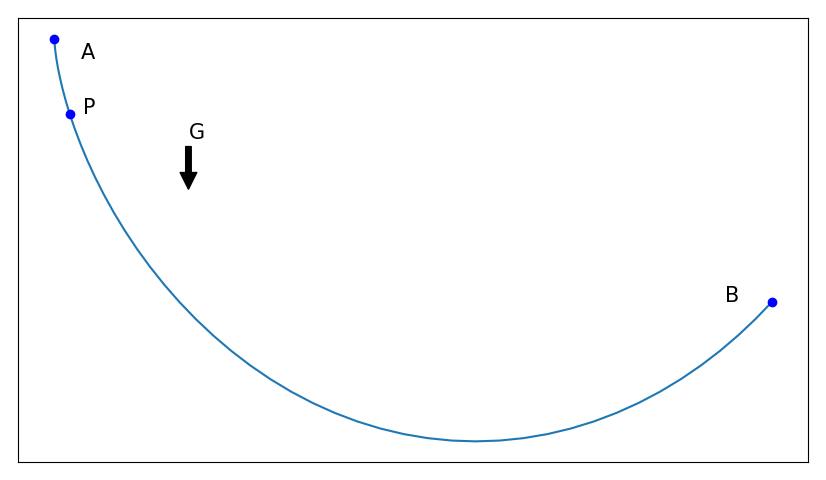
\includegraphics[width=0.9\textwidth]{pearl_on_string.png}
	\caption{Illustration of the Brachistochrone problem}
	\label{fig:brach}
\end{figure}

\subsection{The Period of the Motion}
The total time the body spends moving along the curve is given by a simple integral of infinitesimal time steps
\begin{equation}
T = \int_{t_a}^{t_b}dt.
\end{equation}
Using the velocity and displacement relations $vdt = ds$ gives
\begin{equation}
\label{eq:brachtime2}
T = \int_{A}^{B}\frac{1}{v}ds.
\end{equation}
One such infinitesimal displacement can be decomposed in a Pythagorean manner into $x$ and $y$ parts, $ds = \sqrt{dx^2 + dy^2}$. Inserting into \ref{eq:brachtime2} yields
\begin{equation}
\label{eq:brachtime3}
T = \int_{A}^{B}\frac{1}{v}\sqrt{dx^2 + dy^2} = \int_{x_a}^{x_b}\frac{1}{v}\sqrt{1 + \left(\frac{dy}{dx} \right)^2}dx.
\end{equation}
By assuming conservations of energy $\frac{1}{2}mv^2 + mgy = 0 \to v = \sqrt{-2gy}$ and setting $y'=\frac{dy}{dx}$ equation \ref{eq:brachtime3} becomes
\begin{equation}
T = \int_{x_a}^{x_b} \sqrt{\frac{1+y'^2}{-2gy}}dx.
\end{equation}
If one were to consider this an action integral, then the integrand must therefore be the Lagrangian for the system with $y$ and $y'$ as generalised coordinates
\begin{equation}
L(y,y') = \sqrt{\frac{1+y'^2}{-2gy}}
\end{equation}

\end{document}